\documentclass[11pt]{amsart}
\usepackage[margin=1.15in]{geometry}
\usepackage{amsmath,amssymb,amsthm}
\usepackage{booktabs}
\usepackage{graphicx}
\usepackage[hidelinks]{hyperref}
\usepackage{microtype}

\newtheorem{theorem}{Theorem}[section]
\newtheorem{proposition}[theorem]{Proposition}
\newtheorem{lemma}[theorem]{Lemma}
\theoremstyle{remark}
\newtheorem{remark}[theorem]{Remark}
\theoremstyle{definition}
\newtheorem{definition}[theorem]{Definition}

\newcommand{\Q}{\mathbb{Q}}
\newcommand{\R}{\mathbb{R}}
\newcommand{\ran}{r_{\mathrm{an}}}
\DeclareMathOperator{\supp}{supp}

\title[Optimal windowed test functions for analytic rank bounds]{Optimal windowed test functions for bounding\\ analytic ranks of elliptic curves}
\author{Sabrina Hackfort}
\address{Independent researcher (MEGALODON Research), Germany}
\email{meg.depth@proton.me}
\thanks{ORCID: 0009-0007-7458-2487}
\date{October 2026 \quad (draft v0.5)}

\IfFileExists{board_macros.tex}{\newcommand{\BoardAbstract}{On all 395 leaderboard curves of rank $24$--$31$, with primes below $10^{9}$, the optimised kernel certifies the rank of 362 curves and the fixed kernel of 349; where both succeed the fixed kernel needs a median of 3.9 times as many primes.}
\newcommand{\BoardBrief}{On the 395 leaderboard curves of rank $24$--$31$ ($p<10^{9}$) the optimised kernel certifies 362 ranks, the fixed kernel 349; 13 only by the optimised kernel, none only by the fixed one (Section~\ref{sec:board}).}
\newcommand{\BoardDetail}{On 33 curves neither kernel reaches the target with $p<10^{9}$; on 33 of them the certified bound of the optimised kernel is the smaller one; their certified bounds at the cap are listed in the repository.}
}{%
  \newcommand{\BoardAbstract}{[board results: run scripts/make\_board.py]}%
  \newcommand{\BoardBrief}{[board results: run scripts/make\_board.py]}\newcommand{\BoardDetail}{}\newcommand{\BoardTrend}{}}
\begin{document}

\begin{abstract}
Assuming the Generalized Riemann Hypothesis, the explicit formula for the $L$-function of an elliptic curve $E/\Q$ bounds the analytic rank of $E$ in terms of the traces $a_p$ for $p < e^{2L}$, for any admissible test function supported on a window $[-L,L]$. In rank computations this test function is usually fixed in advance, typically to a Fej\'er-type kernel; optimising it for an individual $L$-function goes back to Booker, and an earlier test on quadratic twists of rank about $7$ found the gain to be small. We choose, for each individual curve, the test function that minimises the resulting bound within a finite-dimensional space supported on $[-L,L]$, certify the result, and measure the gain systematically, up to the current record curves. The minimiser is the solution of a linear system with the Gram matrix of the Weil quadratic form of $E$, and the optimal bound equals the reciprocal of the corresponding reproducing kernel at the central point, which we call the \emph{radix Riemanniana} of $E$. Because the Fej\'er-type kernel lies in this space, the optimised bound is never weaker. We certify every bound with ball arithmetic, check the prime-side evaluation against the zero side computed independently from the zeros of $L(E,s)$, and benchmark against the fixed kernel on $1642$ curves from Cremona's tables, $2500$ curves from the Stein--Watkins database and a set of curves with conductors up to $3\cdot 10^{16}$. Depending on the sample and on the stopping criterion, the number of primes required to pin down the analytic rank decreases by $8$--$23\%$ in aggregate. For individual curves of large conductor the decrease ranges from $0\%$ to $43\%$. Within each sample the gain is largest at rank $0$ and decreases with the rank; it grows again, and by a much larger factor, in the regime of large rank and large conductor where the computation is most expensive. On the smallest-conductor curves of rank $28$--$31$ in the ICARM leaderboard the optimised kernel needs $84$--$85\%$ fewer primes to certify the rank. For the current record, the rank-$32$ curve \#4239 of Elkies, Klagsbrun and Li, it certifies $\ran\le32$ under GRH with $2.53\cdot10^{9}$ primes --- the first upper bound for this curve --- and hence $\ran=32$ under GRH and BSD, while the fixed kernel, certified at $L=12.40$ with $2\,481\,819\,193$ primes, is still $0.39$ above the target. \BoardAbstract{} We validate the fixed-kernel baseline by reproducing every published value of Bober and of Klagsbrun, Sherman and Weigandt with an independent implementation.
\end{abstract}

\maketitle

\section{Introduction}

Let $E/\Q$ be an elliptic curve of conductor $N$ and let $\ran(E)$ be the order of vanishing of $L(E,s)$ at the central point. Under the Generalized Riemann Hypothesis (GRH), Mestre's explicit-formula method~\cite{Mestre} bounds $\ran(E)$ from above by a quantity computed from the traces of Frobenius $a_p$ for $p$ below a cutoff. Bober~\cite{Bober} made this practical with a Fej\'er-type test function, and Klagsbrun, Sherman and Weigandt~\cite{KSW} used the same function to bound the analytic rank of
the Elkies curve by $28$ under GRH. Their accompanying result that its Mordell--Weil rank equals $28$
rests on computing the $2$-ranks of class groups of associated cubic fields, not on the explicit
formula; the method discussed here bounds the analytic rank only. In these works the shape of the test function is fixed, and only its support (the cutoff) is varied.

This note asks a simple question: \emph{for a given curve and a given cutoff, which test function gives the best bound?} Within any finite-dimensional space of admissible functions supported on $[-L,L]$ the answer is explicit. The explicit formula expresses the bound as a ratio of a quadratic form (the Weil form of $E$, evaluated through the $a_p$) to the square of a linear functional. The minimiser is therefore obtained from one linear solve with a Gram matrix. The optimal value is the reciprocal of the reproducing kernel at $0$ of the space equipped with the Weil inner product.

\subsection*{What is known, and what is new}
The Weil quadratic form restricted to functions supported on a finite interval, and its Gram matrices with respect to a basis, have been studied for the Riemann zeta function by Yoshida~\cite{Yoshida}, by Connes, Consani and Moscovici~\cite{CCM}, by Suzuki~\cite{Suzuki} via screw functions and de Branges spaces, and recently by Shi~\cite{Shi} as finite ``Prime--Weil matrices''. Reproducing-kernel methods for Fourier optimisation problems attached to \emph{families} of $L$-functions, where the input is the limiting one-level density rather than data of an individual $L$-function, are due to Carneiro, Chirre and Milinovich~\cite{CCMil}.

Optimising the test function for an \emph{individual} $L$-function is not new. Booker~\cite[\S3]{Booker} writes the explicit-formula sum over zeros as a positive definite quadratic form in the coefficients of a finite family of test functions and minimises it under a linear normalisation by inverting the matrix, in order to locate zeros of Artin $L$-functions. Watkins, Donnelly, Elkies, Fisher, Granville and Rogers~\cite[\S7]{Watkins} applied this extension to analytic-rank bounds for quadratic twists and found the improvement to be small, typically about $0.05$ (for example $7.138$ to $7.090$ with $10$ basis functions, $7.089$ with $40$), and therefore used the fixed kernel. Proposition~\ref{prop:opt} below is the same minimisation in a Legendre basis on the window. We thank the literature for this and claim no novelty for the principle.

What this note adds is (i) certified output for every bound, (ii) a systematic measurement of the gain against the fixed kernel on several thousand curves, and (iii) the observation that the gain, small in the range tested in~\cite{Watkins}, becomes large exactly on curves of high rank and large conductor, where these computations are most expensive. On the ICARM high-rank leaderboard this turns into certified upper bounds for curves where none were known, including the current rank-$32$ record (Section~\ref{sec:records}).

\subsection*{Results in brief}
\begin{itemize}
\item The optimised bound is never weaker than the fixed-kernel bound at the same cutoff (Proposition~\ref{prop:dominate}). This is a consequence of the construction, not an empirical finding. The empirical question is \emph{how much} it gains.
\item Every reported bound is certified rigorously: in Arb ball arithmetic, or, on the leaderboard
sweep, with the prime sum in outward-rounded interval arithmetic and the remaining terms in Arb. In
the benchmark files of Sections~\ref{sec:bench} and~\ref{sec:valid} the two endpoints of each
enclosure coincide when printed as doubles, because at those prime counts the radius falls below
double precision; the certified decision is the comparison of the upper endpoint with the target. No certified bound in our tests contradicts the rank recorded for the curve.
\item The prime-side value of the Weil form agrees with the zero-side value computed from the zeros of $L(E,s)$. The discrepancy halves with each doubling of the height up to which zeros are included (Section~\ref{sec:zeros}).
\item The number of primes needed to determine the analytic rank (Section~\ref{sec:bench}) decreases in aggregate by $8.3$--$15.2\%$ (Cremona, $N<4.1\cdot 10^5$) and by $17.0$--$22.7\%$ (Stein--Watkins, $4.4\cdot10^6\le N\le 7.5\cdot 10^9$), depending on the stopping criterion. For individual curves of conductor up to $5\cdot 10^{15}$ the decrease ranges from $0\%$ to $43\%$.
\item On curves of record rank (Section~\ref{sec:records}) the gain is much larger. For the smallest-conductor curves of ranks $28$--$31$ in the ICARM leaderboard, the number of primes needed for a bound below $r+2$ drops by a factor of about $6.5$. For the bound below $r+1$ the fixed kernel fails for three of the four curves with all primes below $10^9$, while the optimised kernel succeeds with between $2.3\cdot10^5$ and $1.3\cdot10^7$ primes. On the historic record curves $E_{20}$--$E_{27}$ the factor is $2$--$3.5$.
\item For the current record curve \#4239 (rank $\ge32$) the optimised kernel certifies $\ran\le32$ under GRH with all $2\,529\,822\,599$ primes below $6.02\cdot10^{10}$ --- and $\ran=32$ under GRH and BSD, using the $32$ independent points of the leaderboard. The fixed kernel does not reach the target: its certified bound at $L=12.40$, with
$2\,481\,819\,193$ primes, is $[34.39360281\pm4.6\cdot10^{-9}]$ (Section~\ref{sec:4239}).
\item \BoardBrief
\item The fixed-kernel baseline is exactly Bober's method: an independent implementation of Bober's formula reproduces all seven published values in~\cite{Bober,KSW}; it agrees with our floating-point evaluation
to $10^{-6}$, the precision to which we tabulate it, and lies inside our Arb enclosures, whose radii are
below $10^{-12}$ (Section~\ref{sec:valid}).
\end{itemize}

\section{The explicit formula and rank bounds}

Write $L(E,s)=\sum_{n\ge1} a_n n^{-s-1/2}$ so that the central point is $s=1/2$, and put
\[
\Lambda(E,s) = N^{s/2}(2\pi)^{-s}\,\Gamma(s+\tfrac12)\,L(E,s), \qquad \Lambda(E,s)=\pm\Lambda(E,1-s).
\]
For $p\nmid N$ let $\alpha_p,\beta_p$ be defined by $\alpha_p+\beta_p=a_p/\sqrt p$, $\alpha_p\beta_p=1$, and set $c_{p^k}=\alpha_p^k+\beta_p^k$. For $p\mid N$ set $c_{p^k}=(a_p/\sqrt p)^k$ (so $c_{p^k}=0$ for additive reduction). Then $-\frac{L'}{L}(E,s)=\sum_{n\ge2}\Lambda(n)c_n n^{-s}$ in the normalisation above.

Let $f\colon\R\to\R$ be even, bounded and supported in $[-L,L]$. Put $g=f*f$, so that $g$ is even and supported in $[-2L,2L]$, and
\[
\hat f(r)=\int_{\R} f(x)e^{irx}\,dx,\qquad h(r)=\hat g(r)=\hat f(r)^2 .
\]
Writing the nontrivial zeros as $\rho=\tfrac12+i\gamma$ (with multiplicity), the explicit formula reads
\begin{equation}\label{eq:explicit}
\sum_{\gamma} h(\gamma) \;=\; g(0)\log\frac{N}{4\pi^2}
\;+\;2\Big[-\gamma_{\mathrm E}\,g(0)+\int_0^{\infty}\frac{g(0)-g(u)}{e^{u}-1}\,du\Big]
\;-\;2\sum_{n\ge 2}\frac{\Lambda(n)\,c_n}{\sqrt n}\,g(\log n),
\end{equation}
where $\gamma_{\mathrm E}$ is Euler's constant. Only prime powers $n<e^{2L}$ contribute. We denote the right-hand side by $W_E(f)$.

\begin{lemma}\label{lem:bound}
Assume GRH for $L(E,s)$. Then for every nonzero $f$ as above,
\[
\ran(E)\;\le\;\frac{W_E(f)}{\hat f(0)^2}.
\]
\end{lemma}
\begin{proof}
Under GRH every $\gamma$ is real. Since $f$ is real and even, $\hat f$ is real, so $h(\gamma)=\hat f(\gamma)^2\ge0$. The central zero contributes $\ran(E)\,\hat f(0)^2$ to the left-hand side of~\eqref{eq:explicit}, and every other term is nonnegative.
\end{proof}

\begin{remark}
For $f=\mathbf 1_{[-L,L]}$ one has $g(u)=(2L-|u|)_+$ and $h(r)=4\sin^2(Lr)/r^2$. Up to scaling, this is the Fej\'er-type test function used in~\cite{Bober,KSW}. We call the resulting bound $B_{\mathrm{std}}(L)$. With $L=\pi\Delta$ it coincides with Bober's $\sum_\gamma f(\gamma;\Delta)$: $\hat f(r)^2/\hat f(0)^2=(\sin(\Delta\pi r)/(\Delta\pi r))^2$, the conductor term becomes $\log(\sqrt N/2\pi)/(\pi\Delta)$, and the archimedean term evaluates to Spicer's closed form $-\gamma_{\mathrm E}/(\pi\Delta)+\big(\pi^2/6-\operatorname{Li}_2(e^{-2\pi\Delta})\big)/(2\pi^2\Delta^2)$ quoted in~\cite{KSW}.
\end{remark}

\section{The optimal window kernel}

The map $f\mapsto W_E(f)$ is a quadratic form, $W_E(f)=\mathcal B_E(f,f)$, where $\mathcal B_E$ is obtained from~\eqref{eq:explicit} by replacing $g=f*f$ with the symmetrised correlation of two functions. Fix the basis
\[
b_k(x)=P_{2k}(x/L)\,\mathbf 1_{[-L,L]}(x),\qquad 0\le k<K,
\]
of even polynomials on the window, where $P_m$ is the Legendre polynomial of degree $m$. Let $G_{ij}=\mathcal B_E(b_i,b_j)$ be the Gram matrix and $v_i=\hat b_i(0)=\int b_i$, so that $v=(2L,0,\dots,0)$. For $f=\sum c_k b_k$ we have $W_E(f)=c^{\mathsf T}Gc$ and $\hat f(0)=v^{\mathsf T}c$.

\begin{proposition}\label{prop:opt}
If $G$ is positive definite, the minimum of $W_E(f)/\hat f(0)^2$ over nonzero $f$ in $\mathrm{span}(b_0,\dots,b_{K-1})$ equals
\[
B_{\mathrm{rad}}(L)=\frac{1}{v^{\mathsf T}G^{-1}v},
\]
and is attained at $c^\ast=G^{-1}v/(v^{\mathsf T}G^{-1}v)$.
\end{proposition}
\begin{proof}
Minimise $c^{\mathsf T}Gc$ subject to $v^{\mathsf T}c=1$ (Lagrange multipliers, or Cauchy--Schwarz in the inner product $\langle x,y\rangle=x^{\mathsf T}Gy$).
\end{proof}

Since $v=\Phi(0)$, the quantity $v^{\mathsf T}G^{-1}v$ is the value at the central point of the following kernel.

\begin{definition}[Radix Riemanniana]\label{def:radix}
Let $\Phi(z)=(\hat b_0(z),\dots,\hat b_{K-1}(z))^{\mathsf T}$. For an elliptic curve $E/\Q$ and a window $[-L,L]$, the \emph{radix Riemanniana} of $E$ (of order $K$) is the kernel
\[
\mathcal R_{E,L}(w,z)\;=\;\Phi(w)^{\ast}\,G^{-1}\,\Phi(z),
\]
that is, the reproducing kernel of the space $\{\hat f: f\in\mathrm{span}(b_k)\}$ equipped with the Weil inner product $\mathcal B_E$. It is built from the Gamma factor, the conductor and the primes $p<e^{2L}$ alone, without reference to the zeros of $L(E,s)$. The optimal bound of Proposition~\ref{prop:opt} is
\[
B_{\mathrm{rad}}(L)=\frac{1}{\mathcal R_{E,L}(0,0)}.
\]
\end{definition}

\begin{remark}
As $K\to\infty$ the radix Riemanniana is the window analogue, for $L(E,s)$, of the reproducing kernels of the Hilbert spaces of entire functions attached to the Weil form of $\zeta$ in~\cite{Suzuki}. The name and the construction from prime data go back to the author's work on Weil positivity for $\zeta$.
\end{remark}

\begin{proposition}\label{prop:dominate}
For every $L$ with $G$ positive definite, $B_{\mathrm{rad}}(L)\le B_{\mathrm{std}}(L)$.
\end{proposition}
\begin{proof}
$\mathbf 1_{[-L,L]}=b_0$ lies in the span, so $B_{\mathrm{std}}(L)$ is one of the values minimised over in Proposition~\ref{prop:opt}.
\end{proof}

Positive definiteness of $G$ holds under GRH: $W_E(f)=\sum_\gamma\hat f(\gamma)^2\ge0$, and it
vanishes only if $\hat f$ vanishes on the whole zero set; since $\hat f$ is entire of exponential type
$2L$ while the zeros of $L(E,s)$ have counting function $\sim(T\log T)/\pi$, this forces $f=0$. In practice we simply attempt a Cholesky factorisation and discard the window if it fails. Note that \emph{the certificate in Section~\ref{sec:cert} does not depend on optimality or on positive definiteness}: it evaluates $W_E(f)$ for the specific $f$ that was found.

\begin{figure}[h]
\centering
\IfFileExists{surface.pdf}{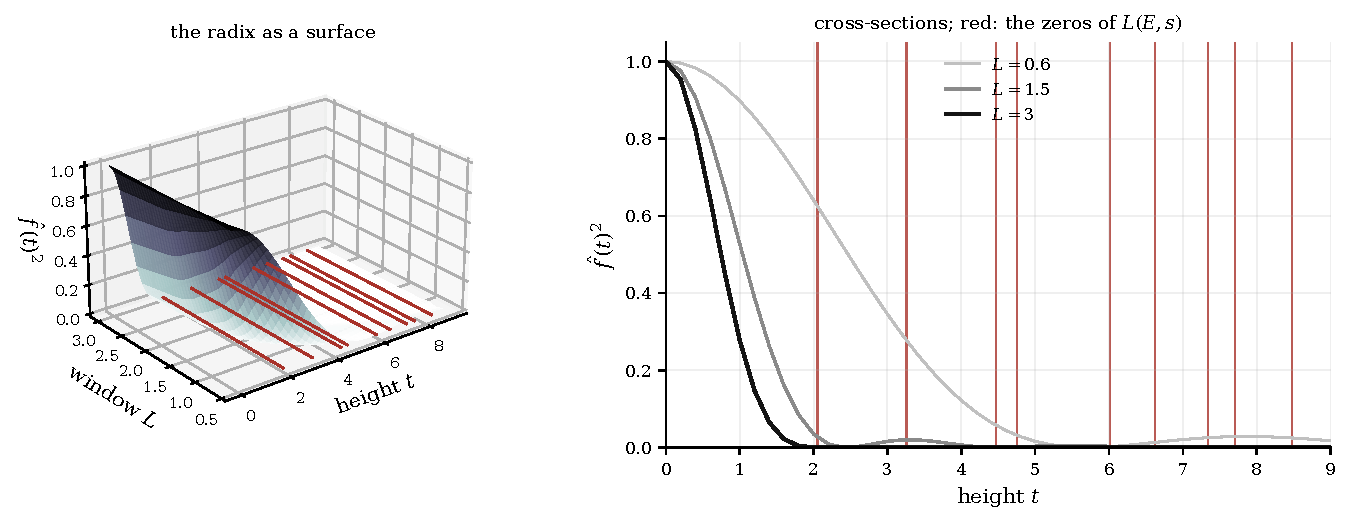
\includegraphics[width=\textwidth]{surface.pdf}}{\fbox{figure \texttt{surface.pdf}: run \texttt{scripts/radix\_surface.py} then \texttt{scripts/plot\_surface.py}}}
\caption{The radix Riemanniana of $5077a1$ (rank $3$, $N=5077$): the optimal kernel $\hat f(t)^2$,
normalised to $\hat f(0)=1$, over the height $t$ and the window $L$, with the zeros of $L(E,s)$ in
red. As the window widens the kernel concentrates at the central point and pulls away from the
zeros; the bound $1/\mathcal R_{E,L}(0,0)$ falls from $5.4241$ at $L=0.6$ to $3.0000$ at $L=3$, the
rank of the curve. Computed from the same Gram matrices as the bounds, by polarisation of the form
implemented in \texttt{scripts/certify.py}.}
\label{fig:surface}
\end{figure}

\section{Certification}\label{sec:cert}

The optimisation is carried out in double precision. The resulting coefficients are converted to exact rationals $c_k\in\Q$, and $L$ is taken to be an exact decimal. For this fixed $f=\sum c_k b_k$ we evaluate $W_E(f)/\hat f(0)^2$ rigorously in ball arithmetic (Arb~\cite{Arb} via \texttt{python-flint}, $256$-bit precision):
\begin{enumerate}
\item On $[0,2L]$, $g=f*f$ is a polynomial with rational coefficients. We compute it exactly in $\Q[u]$ and obtain $\hat f(0)$ exactly.
\item The archimedean integral is split at $u=1/4$. On $[0,1/4]$ we integrate $(g(0)-g(u))/u$ against the Bernoulli expansion $u/(e^u-1)=\sum_n B_n u^n/n!$, truncated after $80$ terms. The tail is bounded with $|B_n|/n!\le 4(2\pi)^{-n}$. On $[1/4,2L]$ the integrand is analytic and is integrated rigorously by Arb's certified Gauss--Legendre integration. The constants $\gamma_{\mathrm E}$, $\pi$ and the logarithms are balls.
\item The prime sum runs over all prime powers $n<e^{2L}$. The quantities $\log n$, $\sqrt n$ and $c_n$ are balls computed from the exact integers $a_p$. If the ball for $\log n$ contains $2L$, the window is rejected.
\end{enumerate}
The output is a ball containing $W_E(f)/\hat f(0)^2$. A statement $\ran(E)<r+1$ is recorded only if the upper end of the ball is below $r+1$.

\subsection*{Large prime counts}
For the record curves of Section~\ref{sec:records} the prime sum has up to $2.5\cdot10^9$ terms, and two further tools are used.

\emph{Traces of Frobenius.} The $a_p$ for $p<10^9$ (Sections~\ref{sec:bench}--\ref{sec:valid}) are computed with PARI/GP~\cite{PARI}. Beyond that we use our own implementation of the baby-step giant-step method of Shanks and Mestre on the curve and its quadratic twist: the whole Hasse interval is searched, the parity of $a_p$ is read off from the $2$-torsion of $E(\mathbb F_p)$, and candidate sets from several points are intersected until a single value remains; the program never guesses and aborts otherwise. Every value is finally re-checked on fresh points of $E$ and of its twist before it is written. On \#4239 it reproduces all $50\,847\,534$ values of PARI for $p<10^9$ bit for bit.

\emph{Prime sum.} The sum in step~3 is enclosed by a second, independent implementation in $\mathtt{f64}$ interval arithmetic: every operation is rounded to nearest and widened outward by one unit in the last place, $\log p$ is computed from the exact reduction $p=m2^e$ and a bounded series for $\operatorname{artanh}$, $\log 2$ is an interval checked against Arb, and $g$ enters through its exact Chebyshev coefficients on $[0,2L]$, rounded outward. All other parts of $W_E(f)/\hat f(0)^2$ are still computed in Arb. On every curve on which both were run the two certificates have the same midpoint and the same
verdict; the interval version is about $10$ times faster per core and its enclosures are wider,
far below every margin reported here.

Which of the two is used is decided by the script, not by the prime bound. Tables~\ref{tab:icarm},
\ref{tab:historic} and~\ref{tab:4239}, that is the record and historic curves including \#4239 at
$p<6.02\cdot10^{10}$, are certified in Arb alone (\texttt{highrank/cert\_4239.py},
\texttt{cert\_stream.py}). The board of Section~\ref{sec:board} is certified throughout with the
interval version (\texttt{scripts/cert\_fast.py}), at every prime bound. Its radii are flat at a
median of $2.6\cdot10^{-9}$ for $p<10^6$ through $p<10^9$ --- there the working precision of the
Arb part dominates --- and rise to a median of $6.5\cdot10^{-8}$ (largest $4.9\cdot10^{-7}$) at
$p<10^{10}$, where the $4.5\cdot10^8$ outward-rounded terms of the prime sum take over. On
every one of the $790$ certified board entries the enclosure is separated from the target by at
least $440$ times its own radius (the tightest case is the fixed kernel on \#3871 at $p<10^{10}$:
margin $1.45\cdot10^{-4}$, radius $3.29\cdot10^{-7}$, ratio $440.7$), so the width of the enclosure decides no case.

\section{Validation against the zeros}\label{sec:zeros}

Identity~\eqref{eq:explicit} lets us check the whole pipeline (Rust optimiser $\to$ rational coefficients $\to$ certified prime side) against an independent computation. We compute the zeros $\gamma$ of $L(E,s)$ up to height $T$ with PARI's \texttt{lfunzeros} and evaluate the zero side $\ran\hat f(0)^2+\sum_{0<|\gamma|\le T}\hat f(\gamma)^2$ for the same certified $f$. Since every omitted term is nonnegative, the truncated zero side must lie below the prime side, and the difference must tend to $0$ as $T\to\infty$.

\begin{table}[h]
\centering\small
\begin{tabular}{lcccccc}
\toprule
curve & $\ran$ & $L$ & prime side (certified) & zero side, $|\gamma|\le T$ & $T$ & difference\\
\midrule
37a1     & 1 & 0.40 & 1.9967148280 & 1.9923507969 & 600 & $4.4\cdot10^{-3}$\\
389a1    & 2 & 0.65 & 2.9926821162 & 2.9903944027 & 600 & $2.3\cdot10^{-3}$\\
5077a1   & 3 & 0.90 & 3.9514652620 & 3.9497072474 & 600 & $1.8\cdot10^{-3}$\\
234446a1 & 4 & 1.15 & 4.9323755046 & 4.9292024883 & 300 & $3.2\cdot10^{-3}$\\
\bottomrule
\end{tabular}
\caption{Certified prime side versus zero side, both normalised by $\hat f(0)^2$, for the optimised test function at the cutoff where the bound first drops below $\ran+1$.}
\label{tab:zeros}
\end{table}

For 37a1 the difference is $8.1\cdot10^{-3}$, $4.4\cdot10^{-3}$ and $2.4\cdot10^{-3}$ at $T=300$, $600$ and $1200$ ($446$, $1024$ and $2313$ zeros). It roughly halves with each doubling of $T$, consistent with a truncation tail of order $(\log T)/T$.

\section{Benchmarks}\label{sec:bench}

For each curve we scan $L$ on a grid of step $0.05$ with $K=10$ basis functions. For both $B_{\mathrm{std}}$ and $B_{\mathrm{rad}}$ we record the first $L$ at which the certified bound drops below $\ran+1$ (criterion~A), and the first $L$ at which it drops below $\ran+2$ (criterion~B; together with the root number, this already determines the parity of $\ran$). Cost is measured as the number of primes $p<e^{2L}$ used. Because of the grid, prime counts at the threshold are quantised. Ties are therefore frequent and slightly understate the gain.

\subsection{Cremona's tables}
We take one curve per isogeny class, sampled up to $150$ per rank from three blocks of Cremona's tables~\cite{Cremona} ($61\le N\le 409989$, $1642$ curves, ranks $0$--$3$), We provide $a_p$ for $p<8200$ ($1028$ primes) and cut off at $L\le 4.5$. Table~\ref{tab:cremona} reports the results. In total $6449$ bounds were certified, and none contradicts the rank recorded for the curve.

\begin{table}[h]
\centering\small
\begin{tabular}{lccc}
\toprule
 & curves decided (std / rad) & rad fewer / equal / more & primes saved\\
\midrule
criterion A ($<\ran+1$) & 1573 / 1592 & 559 / 1014 / 0 & 15.2\%\\
criterion B ($<\ran+2$) & 1642 / 1642 & 263 / 1379 / 0 & \phantom{1}8.3\%\\
\bottomrule
\end{tabular}

\smallskip
\begin{tabular}{lcccc}
\toprule
criterion A, by rank & 0 & 1 & 2 & 3\\
\midrule
curves (both decided) & 381 & 450 & 450 & 292\\
primes saved & 18.8\% & 4.3\% & 3.9\% & 4.5\%\\
\bottomrule
\end{tabular}
\caption{Cremona sample. ``Primes saved'' is the pooled ratio
$1-\sum_E P_{\mathrm{rad}}(E)/\sum_E P_{\mathrm{std}}(E)$ over the curves decided by \emph{both}
kernels, that is the total work saved on the sample; it is not the saving on a typical curve. The
median per-curve saving is $0\%$ under both criteria, and a saving occurs at all on $36\%$ (A) and
$16\%$ (B) of the curves --- see the text. ``Fewer / equal / more'' is likewise over the curves
decided by both; ``curves decided'' counts each kernel separately. Under criterion~A the optimised
kernel decides $19$ curves that the fixed kernel does not decide within the same prime bound, and
there is no curve the other way round.}
\label{tab:cremona}
\end{table}

The two figures differ sharply, and the reason is worth stating. On a curve that both kernels
decide with a few dozen primes the prime bound moves in steps of one prime, so the two usually tie;
the median curve of the Cremona sample therefore saves nothing. The pooled figure is carried by the
minority of curves on which the computation is actually expensive. That is the regime the method is
meant for, and Sections~\ref{sec:records} and~\ref{sec:board} are about it; but the aggregate should
not be read as a per-curve expectation.

\subsection{The Stein--Watkins database}
From the Stein--Watkins database~\cite{SW} (files of the 2011 distribution) we sample $250$ curves per (analytic) rank $0,1,2,3,\ge4$ from two groups: general conductors $4.4\cdot10^6\le N\le9.7\cdot10^7$ and prime conductors $3.6\cdot10^9\le N\le7.5\cdot10^9$, giving $2500$ curves in total. We check every conductor and root number with PARI. The ranks in the database are Watkins' numerically determined analytic ranks. We provide $a_p$ for $p<10^5$ ($9592$ primes) and cut off at $L\le5.75$. In total $9105$ bounds were certified, and none contradicts the database rank.

\begin{table}[h]
\centering\small
\begin{tabular}{lccc}
\toprule
 & decided (std / rad) & rad fewer / equal / more & primes saved\\
\midrule
criterion A & 2059 / 2096 & 1269 / \phantom{1}790 / 0 & 17.0\%\\
criterion B & 2466 / 2484 & \phantom{1}871 / 1595 / 0 & 22.7\%\\
\bottomrule
\end{tabular}

\smallskip
\begin{tabular}{lccccc}
\toprule
criterion B, by rank & 0 & 1 & 2 & 3 & $\ge4$\\
\midrule
curves (both decided) & 466 & 500 & 500 & 500 & 500\\
primes saved & 24.7\% & 15.1\% & 5.7\% & 3.1\% & 2.7\%\\
\bottomrule
\end{tabular}
\caption{Stein--Watkins sample. ``Primes saved'' is the pooled ratio as in
Table~\ref{tab:cremona}. The median per-curve saving is $7.0\%$ under criterion~A and $0\%$ under
criterion~B; a saving occurs at all on $62\%$ and $35\%$ of the curves.}
\label{tab:sw}
\end{table}

\subsection{Large conductors and high rank}
Table~\ref{tab:big} lists every curve of an additional test set, including the cases without gain. Prime counts up to $e^{16}$ were handled by streaming the prime sum.

\begin{table}[h]
\centering\small
\begin{tabular}{lrcccc}
\toprule
curve & $N$ & rank & criterion & primes std / rad & saved\\
\midrule
twist of 11a1, $d=10009$     & $1101980891$         & 1 & B & 329 / 302 & 8\%\\
twist of 389a1, $d=10009$    & $38970051509$        & 1 & B & 3523 / 3523 & 0\%\\
twist of 11a1, $d=100049$    & $110107826411$       & 0 & B & 2466 / 2065 & 16\%\\
twist of 5077a1, $d=10009$   & $508614271237$       & 1 & B & 1220 / 1019 & 16\%\\
twist of 389a1, $d=100049$   & $3893813133989$      & 0$^{\ast}$ & B & 17885 / 13613 & 24\%\\
twist of 5077a1, $d=100049$  & $50819766789877$     & 1 & B & 1220 / 1220 & 0\%\\
twist of 389a1, $d=1000033$  & $389025674423621$    & 0$^{\ast}$ & B & 102084 / 77395 & 24\%\\
twist of 5077a1, $d=1000033$ & $5077335087528853$   & 1 & B & 340436 / 195040 & 43\%\\
twist of 11a1, $d=1000033$   & $11000726011979$     & 0 & B & \multicolumn{2}{c}{undecided by both for $L\le7.5$}\\
\midrule
5187563742a1                 & $5187563742$         & 6 & A & 11 / 10 & 9\%\\
$[1,-1,0,-106384,13075804]$  & $249649566346838$    & 8 & A & 21 / 18 & 14\%\\
$[1,-1,0,-135004,97151644]$  & $32107342006814614$  & 9 & A & 32 / 29 & 9\%\\
\bottomrule
\end{tabular}
\caption{Additional curves. Ranks are lower bounds from PARI's \texttt{ellrank} (points). $^{\ast}$Here the 2-descent leaves rank $0$ or $2$ open. The root number $+1$ together with the certified bound $\ran<2$ gives $\ran=0$ under GRH, and hence rank $0$ by Kolyvagin~\cite{Kolyvagin}.}
\label{tab:big}
\end{table}

\section{Validation against published fixed-kernel computations}\label{sec:valid}

To make sure that $B_{\mathrm{std}}$ is \emph{exactly} the method of~\cite{Bober,KSW}, and not a variant of it, we re-implemented Bober's formula~\cite[eq.~(3)]{Bober} directly from the paper, with the archimedean term in Spicer's closed form and without any code shared with our optimiser. Conductors were taken from the ICARM leaderboard~\cite{ICARM}; $\log N$ agrees with~\cite[Table~1]{Bober} to all printed digits. Table~\ref{tab:valid} shows that the independent implementation reproduces every published value we could find. The floating-point $B_{\mathrm{std}}(\pi\Delta)$ of our optimiser agrees with it to $10^{-6}$ on all seven curves, which is the precision to which we tabulate the
independent values. On the three curves certified in Arb the independent value lies inside the enclosure,
which has radius below $10^{-12}$; the difference between the two midpoints is $2.7\cdot10^{-8}$,
$1.6\cdot10^{-7}$ and $2.8\cdot10^{-7}$ and reflects the rounding of the tabulated value, not the
certificate.

\begin{table}[h]
\centering\small
\begin{tabular}{lccccc}
\toprule
curve & $\log N$ & $\Delta$ & published & independent & certified $B_{\mathrm{std}}(\pi\Delta)$\\
\midrule
$E_{20}$ & 170.09 & 2.0 & 21.70~\cite{Bober} & 21.690724 & $[21.6907238431\pm5\cdot10^{-13}]$\\
$E_{21}$ & 196.68 & 2.5 & 22.68~\cite{Bober} & 22.672713 & \\
$E_{22}$ & 182.72 & 2.0 & 23.71~\cite{Bober} & 23.704751 & $[23.7047512825\pm3\cdot10^{-13}]$\\
$E_{23}$ & 205.06 & 2.5 & 24.49~\cite{Bober} & 24.483411 & \\
$E_{24}$ & 219.93 & 2.5 & 25.57~\cite{Bober} & 25.568173 & $[25.5681730272\pm5\cdot10^{-13}]$\\
$E_{27}$ & 287.01 & 3.1 & $<29$~\cite{KSW} & 28.988058 & \\
$E_{28}$ & 325.90 & 3.2 & 31.30~\cite{Bober} & 31.298359 & \\
\bottomrule
\end{tabular}
\caption{Reproduction of published values of $\sum_\gamma f(\gamma;\Delta)$; \cite{Bober} rounds up. $E_{20}$--$E_{24}$, $E_{28}$ are the curves of~\cite{Bober}, $E_{27}$ that of~\cite{KSW}.}
\label{tab:valid}
\end{table}

\section{Curves of record rank}\label{sec:records}

For curves of large rank the cutoff, and with it the number of primes, grows quickly: Klagsbrun, Sherman and Weigandt used $\Delta=4$ (primes up to $e^{8\pi}\approx 8\cdot10^{10}$, about $40$ hours) for the Elkies curve~\cite{KSW}, and the leaderboard record of rank $30$ was certified with $\Delta=4.25$ (primes up to $\approx4\cdot10^{11}$)~\cite{ICARM}. This is where a better test function matters most. The following comparison was suggested by Z.~Klagsbrun.

\subsection*{Setup}
All curves are taken from the ICARM Elliptic Curve Rank Leaderboard~\cite{ICARM} (snapshot of 12 October 2026, $4201$ curves) in their global minimal models; the rank $r$ is the leaderboard's certified lower bound. We recomputed every conductor from local data with PARI and checked that the root number equals $(-1)^r$ in every case, so that a certified bound $B<r+2$ gives $\ran\le r$ under GRH (and rank exactly $r$ under GRH and BSD). We computed $a_p$ for all $p<10^9$ ($50\,847\,534$ primes), scanned $L$ with step $0.01$ and $K=10$ (for $E_{28}$, $K=14$ and $K=20$ give the same values to $10^{-4}$), and certified every reported value with Arb as in Section~\ref{sec:cert}.

\subsection*{Ranks 28--31}
For each rank $28$--$31$ we take the curve of smallest conductor. Table~\ref{tab:icarm} lists the number of primes needed. For the target $r+2$ the optimised kernel reaches it in all four cases with a window shorter by
$\Delta L\approx1.0$, which reduces the prime bound by roughly $e^{2}$. Near $r+1$ the fixed-kernel bound flattens, and the gap becomes much larger.

\begin{table}[h]
\centering\small
\begin{tabular}{lcccccc}
\toprule
 & & & \multicolumn{2}{c}{bound $<r+2$} & \multicolumn{2}{c}{bound $<r+1$}\\
\cmidrule(lr){4-5}\cmidrule(lr){6-7}
ICARM & $r$ & $\log N$ & fixed & optimal & fixed & optimal\\
\midrule
\#3762 & 28 & 242.9 & 122\,776 & \textbf{19\,235} & 21\,600\,954 & \textbf{234\,855}\\
\#3835 & 29 & 265.4 & 316\,068 & \textbf{48\,890} & $>5.08\cdot10^7$ $^{a}$ & \textbf{717\,477}\\
\#3897 & 30 & 279.9 & 387\,811 & \textbf{59\,820} & $>5.08\cdot10^7$ $^{a}$ & \textbf{691\,123}\\
\#3900 & 31 & 325.3 & 4\,340\,969 & \textbf{665\,760} & $>5.08\cdot10^7$ $^{a}$ & \textbf{13\,209\,786}\\
\bottomrule
\end{tabular}
\caption{Number of primes $p<e^{2L}$ at the first certified $L$ (grid step $0.01$). $^{a}$Not reached with all primes $p<10^9$; the certified fixed-kernel bounds at $L=10.36$ are, in the order of the rows, $[30.00290409\pm3.2\cdot10^{-9}]$ for \#3835, $[31.08984065\pm3.1\cdot10^{-9}]$ for \#3897 and $[32.43064260\pm2.5\cdot10^{-10}]$ for \#3900.}
\label{tab:icarm}
\end{table}

\subsection*{The historic record curves}
On the record curves of~\cite{Bober,KSW} the gain is smaller but consistent (Table~\ref{tab:historic}). For $E_{27}$ the minimal fixed-kernel window $L=9.72$ ($\Delta=3.09$) matches the choice $\Delta=3.1$ of~\cite{KSW}. For $E_{28}$ neither kernel reaches a bound below $30$ with $p<10^9$ (at $L=10.36$: $31.092$ fixed, $30.820$ optimal).

\begin{table}[h]
\centering\small
\begin{tabular}{lcccccc}
\toprule
 & $E_{20}$ & $E_{21}$ & $E_{22}$ & $E_{23}$ & $E_{24}$ & $E_{27}$\\
\midrule
fixed, $<r+2$ & 11\,988 & 181\,084 & 11\,988 & 77\,395 & 103\,973 & 15\,078\,540\\
optimal, $<r+2$ & \textbf{5\,515} & \textbf{83\,298} & \textbf{5\,133} & \textbf{23\,068} & \textbf{32\,069} & \textbf{4\,340\,969}\\
optimal, $<r+1$ & 47\,114 & --- & 37\,128 & 353\,398 & 433\,671 & ---\\
\bottomrule
\end{tabular}
\caption{Historic record curves, primes needed (grid step $0.01$, all values certified). The $r+1$ row was
searched only up to $p<6.7\cdot10^6$ ($457\,497$ primes); within that range the fixed kernel reaches no
bound below $r+1$ on any of the six curves, and ``---'' marks the two on which the optimised kernel does
not either. The $r+2$ row was searched over a larger range, up to $1.5\cdot10^7$ primes.}
\label{tab:historic}
\end{table}

\subsection*{The 2026 records}
In August 2026 curves of rank at least $30$ (\#273) and $31$ (\#302) were found by L.~Alp\"oge and A.~Howell~\cite{ICARM}. For \#273 ($\log N=339.35$, root number $+1$) the leaderboard reports a fixed-kernel bound below $32$ with $\Delta=4.25$. The optimised kernel certifies
\[
\ran(\#273)\;\le\;[31.99478129\pm4.5\cdot10^{-9}]\;<\;32
\]
at $L=9.66$, with $13\,461\,681$ primes $p<2.46\cdot10^8$, so $\ran(\#273)\le30$ under GRH and
$\ran=30$ under GRH and BSD. The fixed kernel does not reach $32$ with all primes below $10^9$: its
certified value at $L=10.36$ is $[32.08095018\pm1.5\cdot10^{-9}]$; carried to the cap of the board of
Section~\ref{sec:board} it succeeds at $72\,713\,579$ primes, so the optimised kernel needs $18.5\%$ of
them. The leaderboard entry used the fixed kernel at $\Delta=4.25$ without scanning $L$, that is about
$1.5\cdot10^{10}$ primes; most of the factor $1100$ between that and our $1.3\cdot10^7$ is the scan, not
the optimisation. For \#302 ($\log N=375.22$, root number $-1$) neither kernel reached $33$ with $p<10^9$ (at $L=10.36$:
fixed $[34.02864458\pm1.3\cdot10^{-9}]$, optimal $33.566$), and a fit of the form $A+C/L$ to the optimal
bound suggested $p\lesssim6\cdot10^9$. Extending the computation to $p<10^{10}$ confirms this: the
optimised kernel certifies
\[
 B_{\mathrm{rad}}(\#302)\;=\;[32.9991320\pm7.09\cdot10^{-8}]\;<\;33 ,
\]
so $\ran(\#302)\le31$ under GRH, and $\ran=31$ under GRH and BSD. At the cap the fixed kernel, using $452\,518\,634$ primes against $339\,885\,370$
for the optimised one, is still at $[33.349252\pm4.92\cdot10^{-7}]$; the fit had suggested $p\lesssim3\cdot10^{10}$ for it, which
remains an extrapolation.

\subsection*{The rank-32 record}\label{sec:4239}
On 15 October 2026 Elkies, Klagsbrun and Li added the curve \#4239 of rank at least $32$ to the leaderboard~\cite{ICARM}, a specialisation of a rank-$17$ fibration of the K3 surface of discriminant $1152$, with $\log N=414.086$ and root number $+1$; no upper bound was known. With all primes $p<6.02\cdot10^{10}$ ($a_p$ by the method above, Arb certification):

\begin{table}[h]
\centering\small
\begin{tabular}{lccc}
\toprule
kernel & $L$ & primes $p<e^{2L}$ & certified bound\\
\midrule
optimal & $12.41$ & $2\,529\,822\,599$ & $[33.99820448\pm1.8\cdot10^{-9}]$\\
optimal & $12.40$ & $2\,481\,819\,193$ & $[34.00293607\pm3.0\cdot10^{-9}]$\\
fixed   & $12.40$ & $2\,481\,819\,193$ & $[34.39360281\pm4.6\cdot10^{-9}]$\\
\bottomrule
\end{tabular}
\caption{The record curve \#4239. The first row is the certificate.}
\label{tab:4239}
\end{table}

\begin{figure}[h]
\centering
\IfFileExists{highrank.pdf}{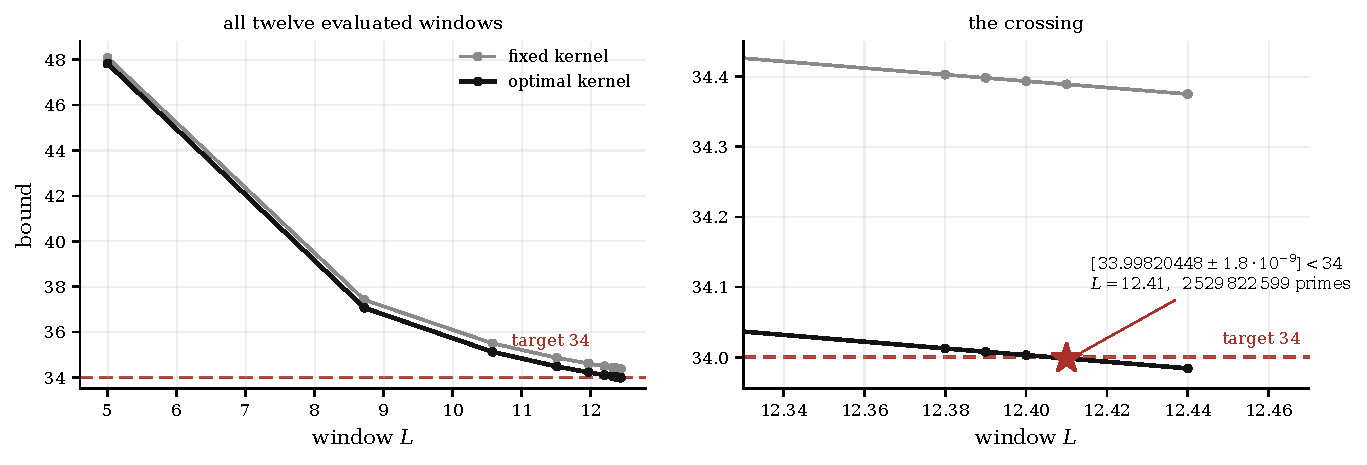
\includegraphics[width=\textwidth]{highrank.pdf}}{\fbox{figure \texttt{highrank.pdf}: run \texttt{scripts/plot\_highrank.py}}}
\caption{The two kernels on \#4239 over the twelve windows at which both were evaluated (floating
point; the entries of Table~\ref{tab:4239} are the certified values at $L=12.40$ and $12.41$). The
optimised bound crosses the target between $L=12.40$ and $L=12.41$; the fixed-kernel bound is still
above $34.37$ at the largest window computed.}
\label{fig:highrank}
\end{figure}

\noindent Hence $\ran(\#4239)\le 33$, and by parity $\ran(\#4239)\le 32$ under GRH; with the $32$ independent points of the leaderboard the rank is exactly $32$ under GRH and BSD. The fixed kernel does not reach the target anywhere in the range computed: its certified bound
at $L=12.40$ is $0.39$ above it (Table~\ref{tab:4239}), and at its largest window $L=12.44$, with
$2\,679\,479\,553$ primes, its floating-point value is still $34.375$. A linear extrapolation in $L$
suggests it would need primes up to about $3\cdot10^{11}$. Doubling the basis from $K=10$ to $K=20$ changes the optimal bound at $p<10^9$ only in the fifth decimal ($35.30281\to35.30276$): within the window the optimisation is saturated, and further gains have to come from more primes.

\section{The ICARM high-rank board}\label{sec:board}
Following a suggestion of Z.~Klagsbrun, we ran both kernels on every curve of the leaderboard with rank lower bound $24$--$31$ (snapshot of 17 October 2026). For each curve the prime bound is raised by factors of $10$ from $10^6$ until both kernels reach the target, or up to a cap; the target is $r+2$; the root number equals $(-1)^r$ for all $395$ curves, so a certified bound below $r+2$ gives $\ran\le r$ under GRH, and $\ran=r$ under GRH and BSD. Every hit is certified as in Section~\ref{sec:cert}; when a kernel does not reach the target below the cap, its certified bound at the largest window is recorded instead. Table~\ref{tab:board} summarises the result by rank; the full list is in the repository (\texttt{highrank/board/}).

\IfFileExists{board.tex}{\begin{table}[!ht]
\centering\small
\begin{tabular}{rrrrrl}
\toprule
rank & curves & optimal & fixed & only optimal & median ratio\\
\midrule
24 & 55 & 55 & 55 & 0 & 3.1\\
25 & 65 & 65 & 65 & 0 & 3.6\\
26 & 43 & 43 & 43 & 0 & 3.6\\
27 & 44 & 43 & 43 & 0 & 4.1\\
28 & 87 & 76 & 74 & 2 & 4.2\\
29 & 50 & 50 & 47 & 3 & 4.7\\
30 & 34 & 34 & 33 & 1 & 5.3\\
31 & 17 & 13 & 12 & 1 & 6.9\\
\midrule
all & 395 & 379 & 372 & 7 & 4.0\\
\bottomrule
\end{tabular}
\caption{ICARM curves of rank $24$--$31$: number of curves on which each kernel certifies $\ran\le r$ under GRH with $p<10^{10}$; ``only optimal'' = certified by the optimal kernel but not by the fixed one; ratio = primes needed by the fixed kernel divided by primes needed by the optimal kernel, over curves where both succeed.}
\label{tab:board}
\end{table}
}{\fbox{Table~\ref{tab:board}: run \texttt{scripts/make\_board.py}}}

\BoardTrend{} \BoardDetail

\section{From primes to time}
\label{sec:time}

Counting primes is the natural measure for this method, because the traces $a_p$ dominate the
cost on curves of large conductor. It is not, however, the same as wall-clock time, and the
difference matters.

In the board computation of Section~\ref{sec:board} the prime bound is raised in powers of ten and
the traces are recomputed from scratch at each stage. On the machine used (one core of an Apple
M-series laptop) the measured times to produce all $a_p$ below $P$ were $0.5$, $1$, $5$, $57$ and
$699$ seconds for $P=10^6,\dots,10^{10}$. The staged search therefore costs the sum of the stages up
to the one that succeeds, not the last stage alone: $762.5$ seconds for a curve carried to the cap,
against $699$ for its final stage, a factor of $1.09$. Aggregated over the board the factor is
$1.11$; for a curve whose last stage is $10^7$ it is $1.5$, because the stage times are not
proportional to $P$.

On a curve run to the cap the traces accounted for $762.5$ of $819$ seconds of wall-clock, that is
$93\%$. The remaining $7\%$ covers the $L$-scan for \emph{both} kernels and the Arb certification at
every stage, and therefore bounds the extra cost of the optimised kernel on that curve. This is a
single measurement, and it is the case most favourable to the traces; for a curve that succeeds at
$10^6$ the certification dominates instead.

Assigning to each kernel the stage at which it first reaches the target, and costing that stage by
the five measured times, gives over the $372$ curves on which both succeed a total trace cost of
$2.49$ hours for the optimised kernel against $5.53$ hours for the fixed one, a factor of $2.22$.
These hours are extrapolated from five timings, not measured curve by curve. The factor is markedly
less than the $4.0$ median of the per-curve prime ratios, and the reason is the granularity of the
search: a curve that needs twice as many primes usually falls in the same decade, so the saving is
not realised. On the $203$ curves where the two kernels fall in different decades the picture is:

\begin{center}\small
\begin{tabular}{lrrr}
\toprule
stages & curves & optimised & fixed\\
\midrule
$10^6\to10^7$ & 79 & $0.5$\,s & $1$\,s\\
$10^7\to10^8$ & 68 & $1$\,s & $5$\,s\\
$10^8\to10^9$ & 43 & $5$\,s & $57$\,s\\
$10^9\to10^{10}$ & 12 & $57$\,s & $699$\,s\\
$10^8\to10^{10}$ & 1 & $5$\,s & $699$\,s\\
\bottomrule
\end{tabular}
\end{center}

\noindent
So even among these the gain in time ranges from a factor of $2$ to a factor of $140$, and on $79$ of
them it is below the median gain in primes. The single curve in the last row is \#4032 of rank $30$.

The honest summary is therefore: in the regime where this method is used at all, the saving in
primes translates into a saving in time of the same order, but only once the prime counts differ
by enough to cross a decade. A search on a finer grid of prime bounds would recover more of it.

\section{Limitations}
\begin{itemize}
\item All bounds assume GRH for $L(E,s)$ and concern the analytic rank. Statements about the algebraic rank additionally use points, the root number and, for $\ran\le1$, the theorems of Gross--Zagier~\cite{GZ} and Kolyvagin~\cite{Kolyvagin}.
\item The basis size is fixed at $K=10$ and the cutoff grid at step $0.05$ ($0.01$ in Sections~\ref{sec:valid} and~\ref{sec:records}). Larger $K$ can only improve $B_{\mathrm{rad}}$, and a finer grid would turn some ties into gains. We have not optimised either choice.
\item Certification uses Arb, and for the prime sum of large instances an independent $\mathtt{f64}$ interval implementation (Section~\ref{sec:cert}); both are written by the author and cross-checked against each other, not formally verified.
\item The gain depends on the curve: on record-rank curves it ranges from a factor of about $2$ ($E_{20}$, $E_{21}$) to $6.4$--$6.5$ (ICARM, ranks $28$--$31$) for a bound below $r+2$; on the board the ratio of prime counts ranges from $1.87$ to $14.95$ over the $372$ curves on which both kernels succeed. For $E_{28}$ we do not reach the target and report only an extrapolation; on the board (Section~\ref{sec:board}) such cases are listed with their certified bound at the cap.
\item Throughout, cost is measured as the number of primes, that is the number of traces $a_p$
required. Section~\ref{sec:time} relates this to wall-clock time; the ratio in time is smaller
than the ratio in primes. The evaluation cost of the kernels themselves is not separated out:
per prime the optimised kernel additionally evaluates Chebyshev moments, and per window it
assembles and factors the Gram matrix, whereas the fixed kernel only accumulates a sum. Both
are contained in the non-$a_p$ share bounded in Section~\ref{sec:time}.
\item Ranks in Section~\ref{sec:records} are certified lower bounds from the leaderboard. Our bounds concern the analytic rank; equality with the algebraic rank requires BSD.
\end{itemize}

\section*{Data and code availability}
Code (Rust optimiser, certification scripts), the sampled curve lists and all certificates are available at \url{https://github.com/sectio-aurea-q/radix-rank} (archived on Zenodo, DOI: \href{https://doi.org/10.5281/zenodo.23299461}{10.5281/zenodo.23299461}). The folders \texttt{validation/} and \texttt{highrank/} contain the independent implementation of Bober's formula and the scripts and certified values for Sections~\ref{sec:valid} and~\ref{sec:records}. Running \texttt{./reproduce.sh quick} re-derives and re-certifies the bounds for seven reference curves in about one minute; \texttt{scripts/rank\_pipeline.sh} and \texttt{scripts/batch\_icarm.py} reproduce Sections~\ref{sec:records} and~\ref{sec:board} from the leaderboard data.

\section*{Acknowledgements}
I thank Zev Klagsbrun for suggesting the comparison on curves of high rank and on the whole leaderboard, for the record curve \#4239, and for forwarding a draft to Jonathan Bober, whose comments I gratefully acknowledge. Curve data were taken from the Elliptic Curve Rank Leaderboard maintained by the NSF Institute
for Computer-Aided Reasoning in Mathematics (ICARM), NSF grant DMS~2425401.

\medskip
\noindent\emph{Tools.} The computations use PARI/GP~\cite{PARI} for curve data and traces of
Frobenius, Arb~\cite{Arb} through \texttt{python-flint} for ball arithmetic, and Rust for the
floating-point optimiser and the interval prime sum. Claude (Anthropic) was used as a tool in
preparing this work. The author takes full responsibility for its content; all results can be
reproduced from the code and certificates in the repository.

\begin{thebibliography}{99}
\bibitem{Arb} F.~Johansson, \emph{Arb: efficient arbitrary-precision midpoint-radius interval arithmetic}, IEEE Trans.\ Comput.\ \textbf{66} (2017), 1281--1292.
\bibitem{Booker} A.~R.~Booker, \emph{Artin's conjecture, Turing's method, and the Riemann hypothesis}, Experiment.\ Math.\ \textbf{15} (2006), no.~4; arXiv:math/0507502.
\bibitem{Bober} J.~W.~Bober, \emph{Conditionally bounding analytic ranks of elliptic curves}, ANTS X, Open Book Ser.\ \textbf{1} (2013), 135--144; arXiv:1112.1503.
\bibitem{CCMil} E.~Carneiro, A.~Chirre, M.~B.~Milinovich, \emph{Hilbert spaces and low-lying zeros of $L$-functions}, arXiv:2109.10844.
\bibitem{CCM} A.~Connes, C.~Consani, H.~Moscovici, \emph{Zeta zeros and prolate wave operators}, arXiv:2310.18423.
\bibitem{Cremona} J.~E.~Cremona, \emph{Algorithms for Modular Elliptic Curves}, 2nd ed., Cambridge Univ.\ Press, 1997; tables at \url{https://github.com/JohnCremona/ecdata}.
\bibitem{GZ} B.~H.~Gross, D.~B.~Zagier, \emph{Heegner points and derivatives of $L$-series}, Invent.\ Math.\ \textbf{84} (1986), 225--320.
\bibitem{ICARM} ICARM, \emph{Elliptic Curve Rank Leaderboard}, \url{https://elliptic-rank.icarm.cloud}, snapshots of 12 and 17 October 2026.
\bibitem{KSW} Z.~Klagsbrun, T.~Sherman, J.~Weigandt, \emph{The Elkies curve has rank 28 subject only to GRH}, Math.\ Comp.\ \textbf{88} (2019), 837--846; arXiv:1606.07178.
\bibitem{Kolyvagin} V.~A.~Kolyvagin, \emph{Euler systems}, in: The Grothendieck Festschrift, Vol.~II, Birkh\"auser, 1990, 435--483.
\bibitem{Mestre} J.-F.~Mestre, \emph{Formules explicites et minorations de conducteurs de vari\'et\'es alg\'ebriques}, Compositio Math.\ \textbf{58} (1986), 209--232.
\bibitem{PARI} The PARI~Group, \emph{PARI/GP}, Univ.\ Bordeaux, \url{https://pari.math.u-bordeaux.fr}.
\bibitem{Shi} Y.~Shi, \emph{Construction of finite Hilbert--P\'olya matrices from Weil's explicit formula}, arXiv:2609.04908.
\bibitem{SW} W.~A.~Stein, M.~Watkins, \emph{A database of elliptic curves---first report}, ANTS V, Lecture Notes in Comput.\ Sci.\ \textbf{2369} (2002), 267--275.
\bibitem{Suzuki} M.~Suzuki, \emph{Weil's quadratic form via the screw function}, arXiv:2606.09096.
\bibitem{Watkins} M.~Watkins, S.~Donnelly, N.~D.~Elkies, T.~Fisher, A.~Granville, N.~F.~Rogers, \emph{Ranks of quadratic twists of elliptic curves}, Publ.\ Math.\ Besan\c{c}on Alg\`ebre Th\'eorie Nr.\ (2014), no.~2, 63--98; doi:10.5802/pmb.9.
\bibitem{Yoshida} H.~Yoshida, \emph{On Hermitian forms attached to zeta functions}, in: Zeta Functions in Geometry, Adv.\ Stud.\ Pure Math.\ \textbf{21} (1992), 281--325.
\end{thebibliography}

\end{document}
